\documentclass{article}
\usepackage[english]{babel}
\usepackage[letterpaper,top=2cm,bottom=2cm,left=3cm,right=3cm,marginparwidth=1.75cm]{geometry}
\usepackage{amsmath}
\usepackage{booktabs}
\usepackage{geometry} % For setting margins
\usepackage{graphicx}
\usepackage{longtable}
\usepackage{float}
\usepackage{setspace}
\usepackage[colorlinks=true, allcolors=blue]{hyperref}
\geometry{a4paper, margin=1in}

\newcommand*{\PathToAssets}{../assets}%
\newcommand*{\PathToOutput}{../output/}%


\title{Replication of The Illiquidity of Corporate Bonds: Project Overview and Table Results}
\author{Group 10: Arthur Ji, Hantao Xiao, Hunter Young, Kathy Zhang}

\begin{document}
\maketitle

\begin{abstract}
Our project set out to replicate Tables 1 (Summary Statistics) and 2 (Measure of Illiquidity) from "The Illiquidity of Corporate Bonds" by Bao, Pan, and Wang (2010). This seminal paper evaluates the impact of illiquidity on corporate bond pricing, employing a novel measure of illiquidity, $\gamma$, for each bond. Focusing on corporate bonds from 2003 to 2009, the study meticulously calculates illiquidity measures and analyzes their valuation effects.
\end{abstract}

\section{Overview}

In the paper, Table 1 generates summary statistics for all corporate bonds and selected samples during 2003 - 2009, and Table 2 calculates illiquidity measure $\gamma$ at both individual bond level and portfolio level. 

In addition to replicating the original tables, we introduced our own supplementary statistics and visualizations of calculated bond illiquidity to further elucidate the data. These enhancements aim to provide a more comprehensive view of the datasets and their implications for corporate bond illiquidity. 

\subsection{Data}

In order to replicate and automate both tables, we leverage four data sources:

\begin{enumerate}
  \item \textbf{WRDS BondRet dataset:} A cleaned database incorporating two feeds: FINRA’s TRACE (Trade Reporting and Compliance Engine) data for bond transactions, and Mergent FISD data for bond issue and issuer characteristics, reported on a monthly basis.
  
  \item \textbf{Daily TRACE panel data:} Maintained by a group of contributors from \href{https://openbondassetpricing.com/}{Open Source Bond Asset Pricing}, this data includes individual level price-relevant data based on FINRA’s TRACE data, reported on a daily basis.
  
  \item \textbf{FINRA’s TRACE data:} The original raw data containing individual level bond characteristics, reported on a trade-by-trade basis.
  
  \item \textbf{MMN-corrected WRDS TRACE data:} The bond-level panel with characteristics adjusted for market microstructure noise, pulled directly from Open Source Bond Asset Pricing, reported on a monthly basis.
\end{enumerate}

\subsection{Replication Results}
Table 1 was reconstructed using data from WRDS BondRet and the original TRACE, including all necessary summary statistics except for trade numbers and sizes, derived from the latter. For Table 2, the daily illiquidity measure leveraged the Daily TRACE panel and MMN-corrected panel, while trade-by-trade illiquidity and bid-ask spreads utilized data from the original TRACE and WRDS BondRet, respectively.

We are successful in replicating the whole process of generating the two tables, applying the filters of sample selection outlined in the paper, and generating similar results compared to the original paper. As informed by our unit tests, our results in the two tables are close to the original paper in terms of absolute values, or, at least, data trends. Additionally, we incorporated the latest data to refresh the tables, capturing recent market dynamics.

\subsection{Challenges}
However, challenges arose due to the limitations of the original datasets. The 2010 paper relied exclusively on TRACE data, which later research suggested might introduce bias due to short-term price reversals. Also, processing the extensive dataset of 346 million trades from 2003 to 2009 was time-intensive. To mitigate these issues, we primarily used pre-processed data from WRDS BondRet and the Daily TRACE panel, which have addressed these reversal effects. This approach, while necessary, occasionally resulted in discrepancies from the original figures due to the different data sources and the exclusion of some transactions recorded in the original TRACE data. We also employed MMN-corrected WRDS TRACE monthly bond data to reconstruct the Table 2 Panel A daily data table, which was a crucial update mentioned on open source bond asset pricing website to adjust for market microstructure noise. After MMN correction, the illiquidity measures are overall lower with higher standard deviation over years.

Updating the results to the current period revealed that the methodology's exclusion of post-Phase 3 bonds (after February 7, 2005) significantly reduced the dataset over time, and certain bond filtering indicates bonds used in 2003-2009 may lose its ability to be included for the updated table, casting doubt on the recent relevance of the illiquidity measures. 


\section{Tables}

\subsection{Table 1 Summary Statistics}

\begin{figure}[htbp]
\centering
\textbf{\large Table 1 from the paper}
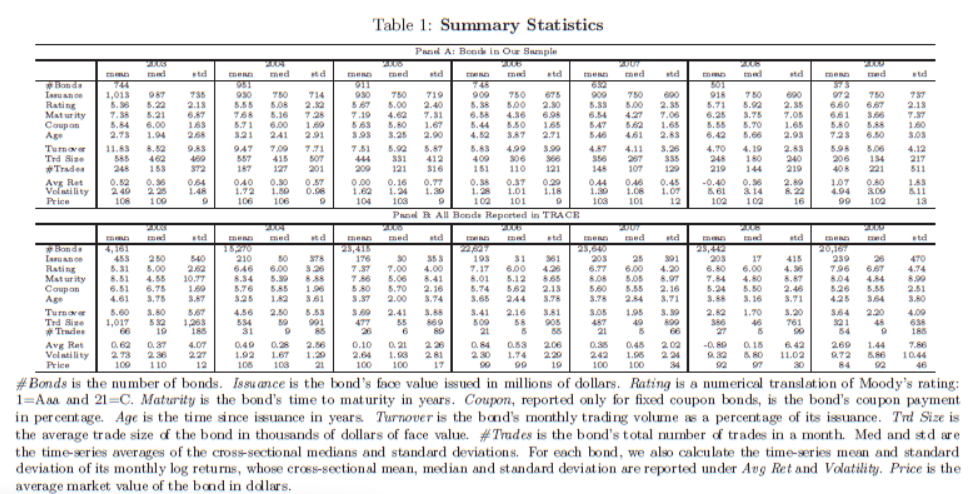
\includegraphics[width=0.75\textwidth]{\PathToAssets/table1_screenshot.jpg}
\end{figure}

\subsubsection{Replicate Tables 1 in the Paper, For period 2003/04-2009/06}
\doublespacing

\subsubsection{Update Table 1 in the Paper, For period 2009/06-Present}
\doublespacing


\subsection{Table 2 Measure of Illiquidity $ \gamma = -\text{Cov}(p_t - p_{t-1}, p_{t+1} - p_t) $ }


\begin{figure}[h]
\centering
\textbf{\large Table 2 in the paper}
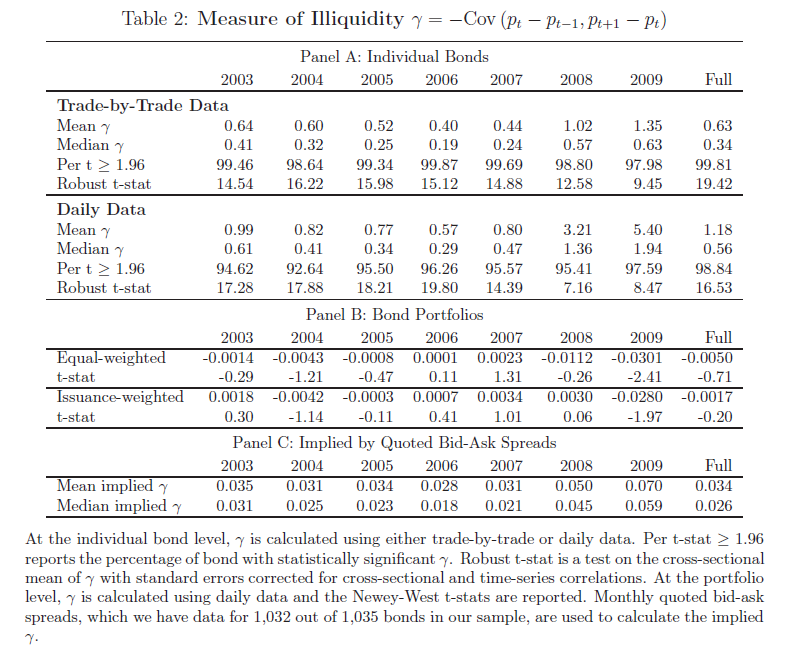
\includegraphics[width=0.75\textwidth]{\PathToAssets/table2_screenshot.jpg}
\end{figure}


\subsubsection{Replicate Table 2 in the Paper, For period 2003/04-2009/06}
\doublespacing
\begin{table}[h]
\centering
\textbf{\large Panel A: Individual Bonds, Trade-by-Trade Data, 2003-2009}
\input{\PathToOutput table2_panelA_trade_by_trade_paper.tex}
\label{table:table2_panelA_trade_by_trade_paper}
\end{table}

\begin{table}[h]
\centering
\textbf{\large Panel A: Individual Bonds, Daily Data, 2003-2009}
\input{\PathToOutput table2_panelA_daily_paper.tex}
\label{table:table2_panelA_daily_paper}
\end{table}

\begin{table}[h]
\centering
\textbf{\large Panel B: Bond Portfolios, 2003-2009}
\input{\PathToOutput table2_panelB_paper.tex}
\label{table:table2_panelB_paper}
\end{table}

\begin{table}[h]
\centering
\textbf{\large Panel C: Implied by Quoted Bid-Ask Spreads, 2003-2009}
\input{\PathToOutput table2_panelC_paper.tex}
\label{table:table2_panelC_paper}
\end{table}


\subsubsection{Update Table 2 in the Paper, For period 2003/04-Present}

\begin{table}[h]
\centering
\textbf{\large Panel A: Individual Bonds, Trade-by-Trade Datas, 2003-Present}
\resizebox{\textwidth}{!}{%
    \input{\PathToOutput table2_panelA_trade_by_trade_new.tex}
}
\label{table:table2_panelA_trade_by_trade_new}
\end{table}

\begin{table}[h]
\centering
\textbf{\large Panel A: Individual Bonds, Daily Data, 2003-Present}
\resizebox{\textwidth}{!}{%
    \input{\PathToOutput table2_panelA_daily_new.tex}
}
\label{table:table2_panelA_daily_new}
\end{table}


\begin{table}[h!]
\centering
\textbf{\large Panel B: Bond Portfolios, 2003-Present}
\resizebox{\textwidth}{!}{%
    \input{\PathToOutput table2_panelB_new.tex}
}
\label{table:table2_panelB_new}
\end{table}


\begin{table}[h!]
\centering
\textbf{\large Panel C: Implied by Quoted Bid-Ask Spreads, 2003-Present}
\resizebox{\textwidth}{!}{%
    \input{\PathToOutput table2_panelC_new.tex}
}
\label{table:table2_panelC_new}
\end{table}


\subsubsection{Table 2 Panel A Daily Data using MMN-Corrected Bond Data}


\begin{table}
\centering
\textbf{\large Panel A: Individual Bonds, MMN-Corrected Bond Data, 2003-2009}
\input{\PathToOutput table2_panelA_daily_mmn_paper.tex}
\label{table:table2_panelA_daily_mmn_paper}
\end{table}


\begin{table}[h!]
\centering
\textbf{\large Panel A: Individual Bonds, MMN-Corrected Bond Data, 2003-Present}
\resizebox{\textwidth}{!}{%
    \input{\PathToOutput table2_panelA_daily_mmn_new.tex}
}
\label{table:table2_panelA_daily_mmn_new}
\end{table}


\subsection{Monthly Bond Illiquidity Summary Statistics}

\begin{table}
\centering
\textbf{\large Monthly Bond Illiquidity Summary Statistics Using Daily Data, 2003-2009}
\input{\PathToOutput illiq_summary_paper.tex}
\label{table:illiq_summary_paper}
\end{table}


\begin{table}[h!]
\centering
\textbf{\large Monthly Bond Illiquidity Summary Statistics Using Daily Data, 2003-Present}
\resizebox{\textwidth}{!}{%
    \input{\PathToOutput  illiq_summary_new.tex}
}
\label{table: illiq_summary_new}
\end{table}


\begin{table}
\centering
\textbf{\large Monthly Bond Illiquidity Summary Statistics Using MMN-Corrected Bond Data, 2003-2009}
\input{\PathToOutput illiq_daily_summary_mmn_paper.tex}
\label{table:illiq_daily_summary_mmn_paper}
\end{table}


\begin{table}[h!]
\centering
\textbf{\large Monthly Bond Illiquidity Summary Statistics Using MMN-Corrected Bond Data, 2003-Present}
\resizebox{\textwidth}{!}{%
    \input{\PathToOutput illiq_daily_summary_mmn_new.tex}
}
\label{table: illiq_daily_summary_mmn_new}
\end{table}


\section{Visualizations}

\subsection{Monthly Illiquidity Per Bond and Average Illiquidity By Year}

\begin{figure}
\centering
\caption{Illiquidity by Year with Mean Illiquidity, 2003-2009}
  \centering
  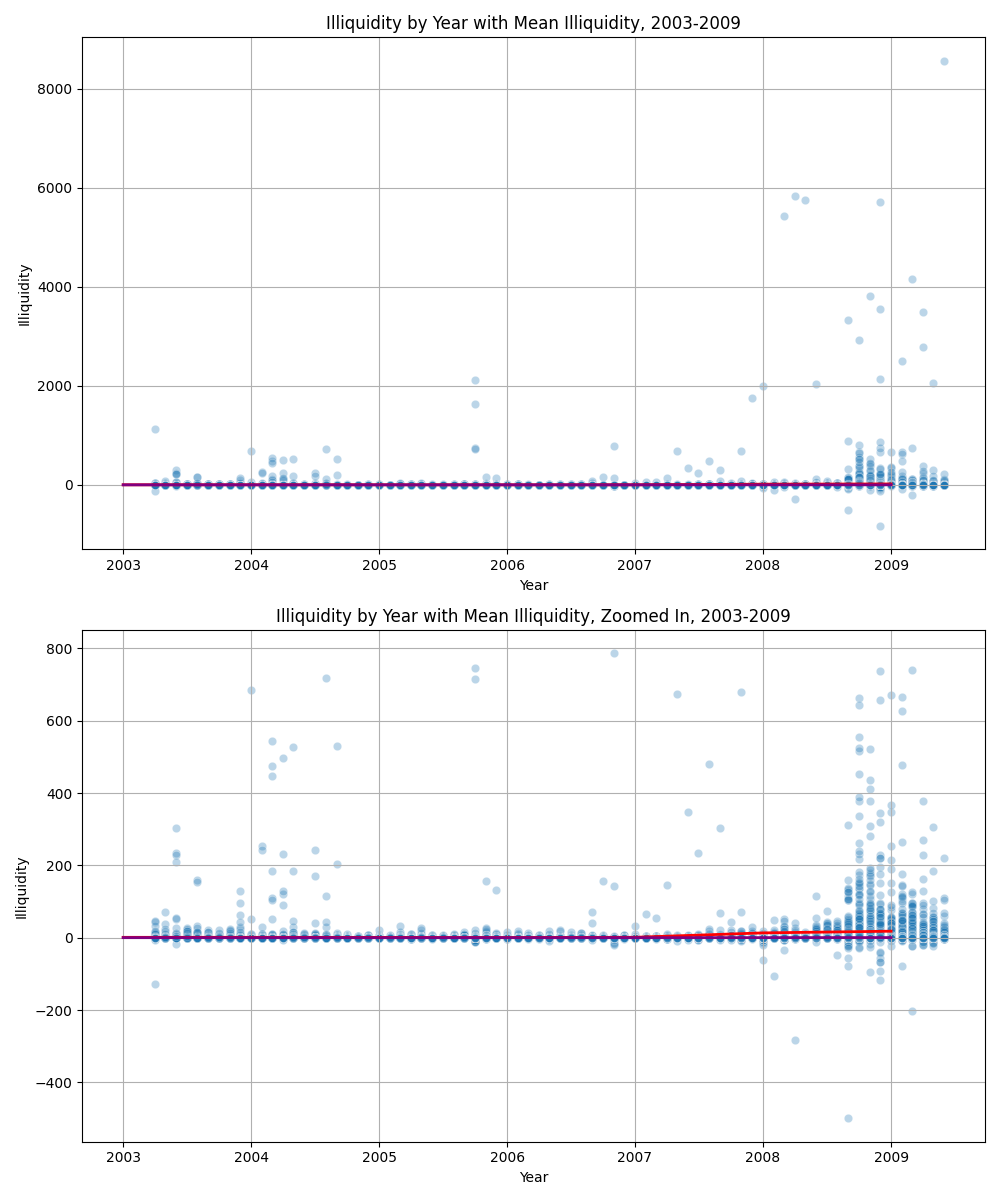
\includegraphics[width=0.75\linewidth]{\PathToOutput/illiq_plot_2003-2009.png}
  % \caption{Average returns}

\label{fig:illiq_plot_2003-2009}
\end{figure}


\begin{figure}
\centering
\caption{Illiquidity by Year with Mean Illiquidity, 2003-Present}
  \centering
  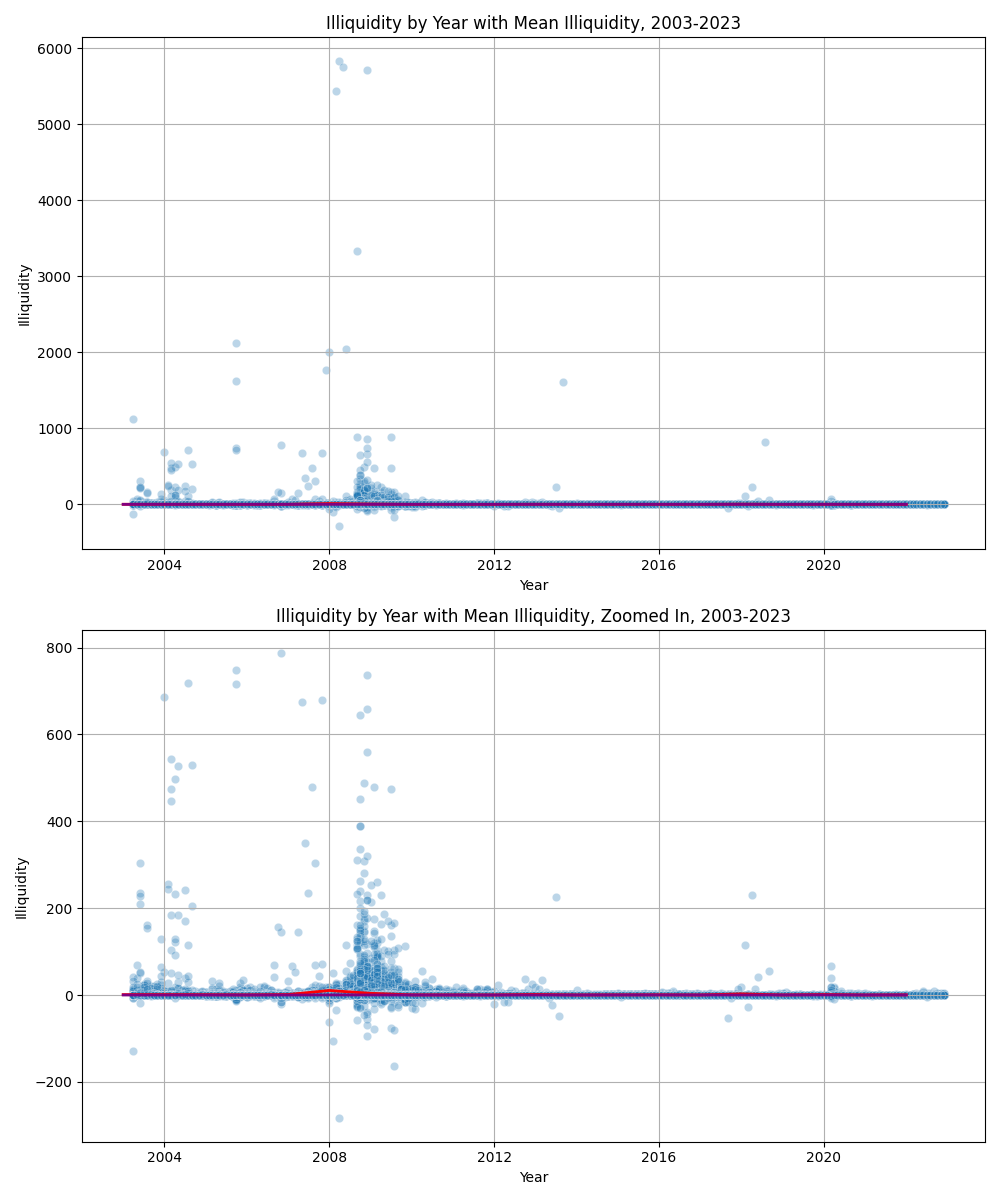
\includegraphics[width=0.75\linewidth]{\PathToOutput/illiq_plot_2003-2023.png}
  % \caption{Average returns}

\label{fig:illiq_plot_2003-2023}
\end{figure}

\end{document}